\section{Elementare Lösungsverfahren}
\subsection{Elementar lösbare Differentialgleichungen}
Eine Differentialgleichung heisst Elementar Lösbar wenn sie in der Form
\begin{equation*}
    y^{\left( n \right)} = f(x)
\end{equation*}
geschrieben werden kann.

Lösungsverfahren: n-mal integrieren.

Beispiel:

\begin{IEEEeqnarray*}{rClr}
    y'' &=&  x^{2} &\hspace{3em} \left|\int dx\right.\\
    \int y'' dx &=& \int x^{2} dx &\\
    y' &=& \frac{1}{3}x^{3}+C_1 &\left|\int dx\right.\\
    y &=& \int\left(\frac{1}{3}x^{3}+C_1  \right)dx &\\
    &=& \frac{1}{12}x^{4}+C_1\cdot x + C_2 &
\end{IEEEeqnarray*}
Zusätzliche Bedingungen: \\
Ordnung 2 $\Rightarrow$ Es braucht 2 RB:
$y\left( 0 \right)=1,~y'\left( 1 \right)=-2$

\begin{eqnarr}
    y\left( 0 \right) &=& C_2 = 1 \\
    y'\left( 1 \right) &=& \frac{1}{3}\cdot 1+C_1 = -2 \\
    &\Rightarrow& \\
    C_1 &=& -2-\frac{1}{3} = -\frac{7}{3} \\
    &\Rightarrow& \\
    y\left( x \right) &=&  \frac{1}{12}x^{4} - \frac{7}{3}x +1
\end{eqnarr}

\subsection{Separierbare Differentialgleichungen}
Eine Differentialgleichung 1.Ordnung heisst separierbar, wenn sie in der Form
\begin{equation*}
    y' = \frac{f(x)}{g(y)}
\end{equation*}
geschrieben werden kann.

Lösungsverfahren:
\begin{IEEEeqnarray*}{rCll}
    y' &=& \frac{dy}{dx} = \frac{f(x)}{g(y)} &\hspace{3em}\left| 
    \begin{array}{c}
    \cdot dx\\
    \cdot g(y)\\
    \end{array} \right.\\
    &\Rightarrow& & \\
    g\left( y \right) dy &=& f\left( x \right) dx & \hspace{3em}\left|\hspace{0.5em} \int \right. \\
    \int g\left( y \right) dy &=& \int f\left( x \right) dx &
\end{IEEEeqnarray*}
und ausrechnen\ldots\\
Die Methode ist einfach, schwierig ist das Erkennen der Separierbarkeit (und
das Integrieren der Funktionen)

\bsp{Spezialfall}
Achtung, wenn $g(y)^{-1}=0$, dann ist die Operation $\cdot g(y)$ nicht erlaubt
$\Rightarrow g(y)^{-1}=0$ muss immer separat überprüft werden.

Beispiel 1:
\begin{IEEEeqnarray*}{rClr}
    y' &=& \frac{3y}{x}&\\
    \frac{dy}{dx} &=& \frac{3y}{x}&\\
    \int\frac{1}{y} \dd{y}&=& \int\frac{3}{x}\dd{x}& y\neq 0\\
    \ln\left( |y| \right) + C_1 &=& 3\cdot\ln\left( |x| \right)+C_2&
    \hspace{2em}C_1,C_2\in\mathbb{R}\\
    \ln\left( |y| \right) &=& 3\cdot\ln\left( |x| \right)+C_3&C_3\in\mathbb{R}\\
    &=& \ln\left( |x|^3 \right)+C_3&\\
    |y| &=&  e^{\ln(|x|^3)+C_3}&\\
    &=&  e^{\ln(|x|^3)}\cdot e^{C_3}&\\
    &=&  x^3 \cdot e^{C_3}&\\
    &=& C_4 \cdot x^3&C_4\in\mathbb{R}^+\\
\end{IEEEeqnarray*}
Was ist wenn $g(y)^{-1}=0$? Dann ist 

Beispiel 2:
\begin{equation*}
    y' = \ln\left( x+y \right)
\end{equation*}
Ist nicht separierbar.

Beispiel 3:
\begin{eqnarr}
    \dot{x} &=& -6x\\
    \frac{dx}{dt} &=& -6x\\
    \int \frac{1}{x} dx &=&  \int -6 dt \\
    \ln x &=&  -6t+C_1 \\
    x &=&  e^{-6t+C_1} = e^{-6t}\cdot \underbrace{e^{C_1}}_{C}\\
    x(t) &=& C\cdot e^{-6t}
\end{eqnarr}



%%%%%%%%%%%%%%%%%%%%%%%%%%%%%%%%%%%%%%%
\subsection{Richtungsfeld}
Für DGL der Form $y'=f(x,y)$\\ (Nur für DGL 1. Ordnung, die nach $y'$
auflösbar sind)

\begin{center}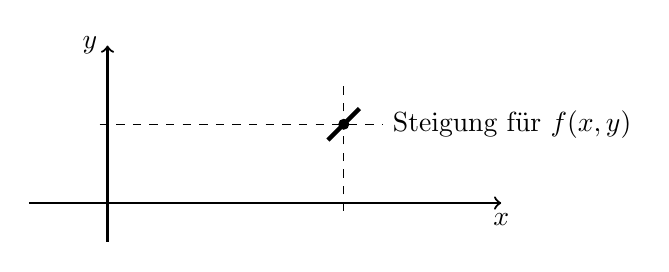
\begin{tikzpicture}
    \draw[thick] (-1,0) -- (0,0) -- (0,-0.5);
    \draw[<->,thick] (5,0) node[below] {$x$} -- (0,0) -- (0,2) node [left] {$y$};
    \draw[dashed] (-0.1,1) --(3.5,1);
    \draw[dashed] (3,-0.1) --(3,1.5);
    \draw[ultra thick] (2.8,0.8) --++ (0.4,0.4);
    \fill (3,1) circle[radius= 0.07];
    \node[right] at (3.5,1) {Steigung für $f(x,y)$};
\end{tikzpicture}\end{center}

\bsp{Beispiel:} $y'=2x$

